\newpage
\begin{center}
  \textbf{\large АННОТАЦИЯ}
\end{center}

В настоящей работе рассматриваются белковые комплексы вида белок-белок, где в качестве компонент комплекса выступают белки, представленные в полноатомном виде. При моделировании процесса образования устойчивого комплекса компонентами при их нековалентном взаимодействии друг с другом возникает необходимость в вычислении энергии такого взаимодействия. Одним из существующих методов для вычисления энергии взаимодействия является использование оценочной функции, которая для заданной пространственной конфигурации компонент позволяет приближенно оценить искомую энергию. В работе приведено описание разработанной оценочной функции и ее оптимизация при помощи Kd-дерева, в которой учитываются силы межатомных взаимодействий, представленные эмпирическими потенциалами Кулона и Леннард-Джонса. Молекулы растворителя в явном виде не рассматриваются, для этого энергия сольватации вычисляется в рамках модели неявного растворителя. Для тестового набора комплексов приведены результаты численных экспериментов, демонстрирующие ускорение результаты вычислений энергии взаимодействия разработанных функций и существующих инструментов.

This work examines protein complexes of the protein-protein type, where the components of the complex are proteins represented in full atomic form. When modeling the process of forming a stable complex, there is a need to calculate the energy of such non-covalent interactions between the components. One of the existing methods for calculating interaction energy is the use of an evaluation function, which approximately estimates the desired energy for a given spatial configuration of the components. The work describes the developed evaluation function and its optimization using a Kd-tree, which takes into account interatomic interaction forces represented by Coulomb and Lennard-Jones empirical potentials. Solvent molecules are not explicitly considered, and the solvation energy is calculated within the framework of an implicit solvent model. Results of numerical experiments for a test set of complexes are presented, demonstrating the acceleration of energy interaction calculations using the developed functions compared to existing tools.

\onehalfspacing
\thispagestyle{empty} 

\newpage
\renewcommand{\contentsname}{\centerline{\large СОДЕРЖАНИЕ}}
\setcounter{page}{4}
\tableofcontents

\newpage
\begin{center}
  \textbf{\large ВВЕДЕНИЕ}
\end{center}
\addcontentsline{toc}{chapter}{ВВЕДЕНИЕ}

В настоящее время разработано множество оценочных функций, которые подразделяются на группы, исходя из принципов их построения. Например, распространено нестрогое деление на эмпирические, статистические и функции на основе силовых полей\cite{ci500731a}. Помимо точности оценки искомой энергии взаимодействия важными критерием выбора оценочной функции является вычислительная сложность процедуры оценки, поэтому при моделировании взаимодействия на больших временных масштабах прибегают к моделям с упрощенным представлением белков\cite{biom10071056}, а также исключают конформационную подвижность, рассматривая компоненты комплекса как <<твёрдые>> тела, совершающие в растворителе только поступательные и вращательные движения.

Существует множество инструментов для оценки энергии взаимодействия, но они, помимо высчитывания энергии, обрабатывают и преобразуют входные данные, выполняют некоторые вычисления, это занимает много времени. Разработанная и оптимизированная в данной работе функция не выполняет лишних вычислений с белком -- работает значительно быстрее других инструментов.

Целями работы являются: разработка, реализация и верификация оценочной функции для учета межмолекулярных взаимодействий в белковых комплекса.
Функция разработана для оценки энергии при моделировании процесса образования белкового комплекса с помощью кинетического метода Монте-Карло\cite{Voter}. В основе метода лежит классическая теория переходного состояния, где в процессе моделирования система движется в сторону наименьшей полной энергии по пути с наименьшими энергетическими барьерами, что позволяет модельной системе на пути к термодинамическому равновесию проходить через последовательность квазиравновесных состояний. Следует отметить, что для моделирования процесса образования комплекса достаточно сформировать оценочную функцию, учитывающую только парные межатомные взаимодействия и влияние растворителя\cite{biom10071056}. 

\newpage
\begin{figure}[h!]
	\centering
	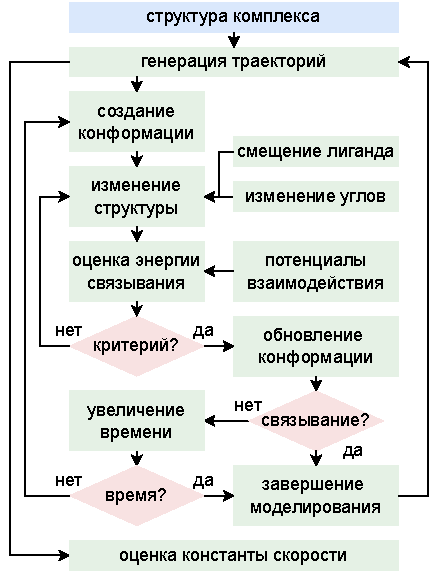
\includegraphics[width=0.6\linewidth]{images/kmc.pdf}
	\caption{Структура комплекса}
	\label{monte}
\end{figure}
